\section{Fundamentação Teórica}
\label{sec:theoretical}

Esta seção apresenta os conceitos fundamentais que embasam esta pesquisa. Está organizada em
quatro partes: conceitos gerais de banco de dados e o modelo relacional; sistemas de bancos de
dados distribuídos; bancos de dados de séries temporais e suas arquiteturas específicas; e
metodologia de benchmarking.

\subsection{Bancos de Dados}

De acordo com~\cite{Ramakrishnan2003}, um banco de dados pode ser definido como uma coleção de
dados que tipicamente descreve as atividades de uma ou mais organizações relacionadas.
Isso abrange desde informações sobre entidades (como estudantes e cursos em uma universidade)
até os relacionamentos entre essas entidades, como as matrículas de alunos em disciplinas
específicas. \cite{Silberschatz2020} acrescenta que o objetivo primário de um sistema de banco de
dados deve ser fornecer uma maneira de armazenar e recuperar informações que seja ao mesmo tempo
conveniente e eficiente.

O gerenciamento desses dados é realizado por um Sistema Gerenciador de Banco de Dados (SGBD),
que é um software projetado para auxiliar na manutenção e uso de grandes coleções de
dados~\citep{Ramakrishnan2003}. A necessidade de tais sistemas cresceu rapidamente, pois a
alternativa de armazenar dados em arquivos planos e escrever código de gerenciamento específico
para cada aplicação produz soluções que não são transferíveis entre aplicações e não oferecem
garantias de integridade ou de acesso concorrente seguro.

Como enfatizado por~\cite{Ramakrishnan2003}, o sucesso de uma organização depende cada vez mais
de sua capacidade de adquirir dados precisos e oportunos sobre suas operações, gerenciar esses
dados de forma eficaz e utilizá-los para analisar e guiar suas atividades. Isso posiciona o banco
de dados como um ativo organizacional estratégico, e não meramente como um componente técnico.
\cite{Silberschatz2020} acrescenta que um banco de dados deve fornecer aos usuários uma visão
abstrata dos dados, ocultando os detalhes de armazenamento e representação para que possa servir
como uma abstração prática para resolução de problemas.

\cite{Ramakrishnan2003} enumeram diversas vantagens dos SGBDs em relação aos sistemas de arquivos
tradicionais: independência de dados (os programas de aplicação são isolados dos detalhes de
representação e armazenamento de dados); acesso eficiente aos dados (por meio de técnicas
sofisticadas de indexação e otimização de consultas); integridade e segurança dos dados (o SGBD
impõe restrições e restringe acessos não autorizados); e suporte para acesso concorrente e
recuperação de falhas.

O modelo relacional, proposto por Codd em 1970, é simples e elegante: um banco de dados é visto
como uma coleção de relações (tabelas com linhas e colunas), uma representação tão intuitiva
que mesmo usuários não especialistas conseguem entender o conteúdo armazenado~\citep{Ramakrishnan2003}.
A estrutura de cada relação consiste em um esquema (nomes dos campos e seus domínios) e uma
instância (o conjunto de tuplas, ou registros). Uma propriedade essencial é que cada relação é
um conjunto de tuplas únicas, garantindo a ausência de registros duplicados. Restrições de
integridade, ou seja, condições especificadas no esquema que restringem os dados armazenáveis,
garantem que apenas instâncias válidas do banco de dados possam ser persistidas. Entre elas,
as restrições de chave primária identificam unicamente as tuplas, enquanto as restrições de
chave estrangeira mantêm a consistência quando informações em uma relação referenciam outra.

O SQL tornou-se o padrão comercial para interação com bancos de dados relacionais.
Como observam~\cite{Ramakrishnan2003}, o SQL é a linguagem comercial mais amplamente utilizada
para SGBDs relacionais, dando suporte não apenas à definição e manipulação de dados, mas também
a consultas complexas. O projeto de banco de dados tipicamente começa com um diagrama
Entidade-Relacionamento (ER) como representação de alto nível, que é então traduzido em um
esquema relacional.

\subsection{Bancos de Dados Distribuídos}

Os bancos de dados distribuídos (BDDs) são a convergência das tecnologias de sistemas de
banco de dados e redes de computadores~\citep{Ozsu2011}.
Os sistemas de banco de dados fornecem os mecanismos de armazenamento, consulta e controle
de integridade dos dados, enquanto as redes de computadores viabilizam a distribuição física
entre múltiplos nós. A tecnologia dos BDDs combina esses dois campos, demonstrando que a
integração de dados não implica necessariamente centralização física.

Para~\cite{Silberschatz2020}, um sistema de banco de dados distribuído é composto por múltiplas
instâncias com bancos de dados locais, cada uma capaz de processar transações locais, ao mesmo
tempo em que executa transações globais que acessam dados em múltiplos locais, exigindo
comunicação entre sítios.

Um banco de dados distribuído é definido como uma coleção de múltiplos bancos de dados
logicamente inter-relacionados, distribuídos por uma rede de computadores~\citep{Ozsu2011}.
O SGBD distribuído (SGBDD) é o software que gerencia esse banco de dados distribuído, tornando
a distribuição transparente para os usuários. Um BDD não é simplesmente uma coleção de arquivos
armazenados em diferentes nós de rede; é um sistema estruturado com um esquema definido,
acessível por meio de uma interface comum.

A arquitetura de um SGBDD pode assumir diversas formas, incluindo cliente/servidor,
ponto-a-ponto e sistemas multibanco~\citep{Ozsu2011}. Em sistemas cliente/servidor, as funções
são divididas entre clientes (que gerenciam a interface do usuário) e servidores (responsáveis
pelo gerenciamento de dados). Em sistemas ponto-a-ponto, todas as máquinas possuem
funcionalidade completa de SGBD e podem se comunicar diretamente. Os sistemas multibanco lidam
com a integração de bancos de dados heterogêneos e autônomos.

Um benefício fundamental dos BDDs é o desempenho melhorado por meio da localidade de dados e
do paralelismo. Como observam~\cite{Ozsu2011}, armazenar dados próximos aos seus pontos de uso
reduz a contenção de CPU e E/S, enquanto o paralelismo pode ser explorado tanto entre consultas
(interqueries) quanto dentro de uma única consulta (intraquery). No entanto, isso traz desafios:
consistência da replicação, sincronização de transações distribuídas e detecção de deadlock
distribuído, como destacado por~\cite{Ozsu2011} e~\cite{Silberschatz2020}. O objetivo mais
importante da tecnologia de banco de dados, como argumentam~\cite{Ozsu2011}, é a integração,
não a centralização.

\subsection{Bancos de Dados de Séries Temporais}
\label{sec:tsdb-theory}

Os Bancos de Dados de Séries Temporais (BDSTs) são uma categoria especializada de sistemas
de armazenamento projetados para lidar com dados registrados como uma sequência de valores,
cada um associado a um instante de tempo específico. De acordo com~\cite{Ozsu2011}, uma série
temporal é um conjunto de valores de atributos ao longo de um período de tempo. Essa
característica fundamental diferencia os BDSTs dos bancos de dados de uso geral: eles são
otimizados para consultas baseadas em intervalos de tempo, oferecendo desempenho superior para
esse padrão de acesso.

Registros meteorológicos, indicadores econômicos e métricas de saúde de pacientes são todos
dados de séries temporais. Os dados de séries temporais também incluem métricas de servidores,
monitoramento de desempenho de aplicações, dados de rede, dados de sensores, eventos, cliques
e muitos outros tipos de dados analíticos~\citep{InfluxDataTimeSeries}.
A Figura~\ref{fig:temporal_data} ilustra uma série temporal de medições meteorológicas.

\begin{figure}[ht]
  \centering
  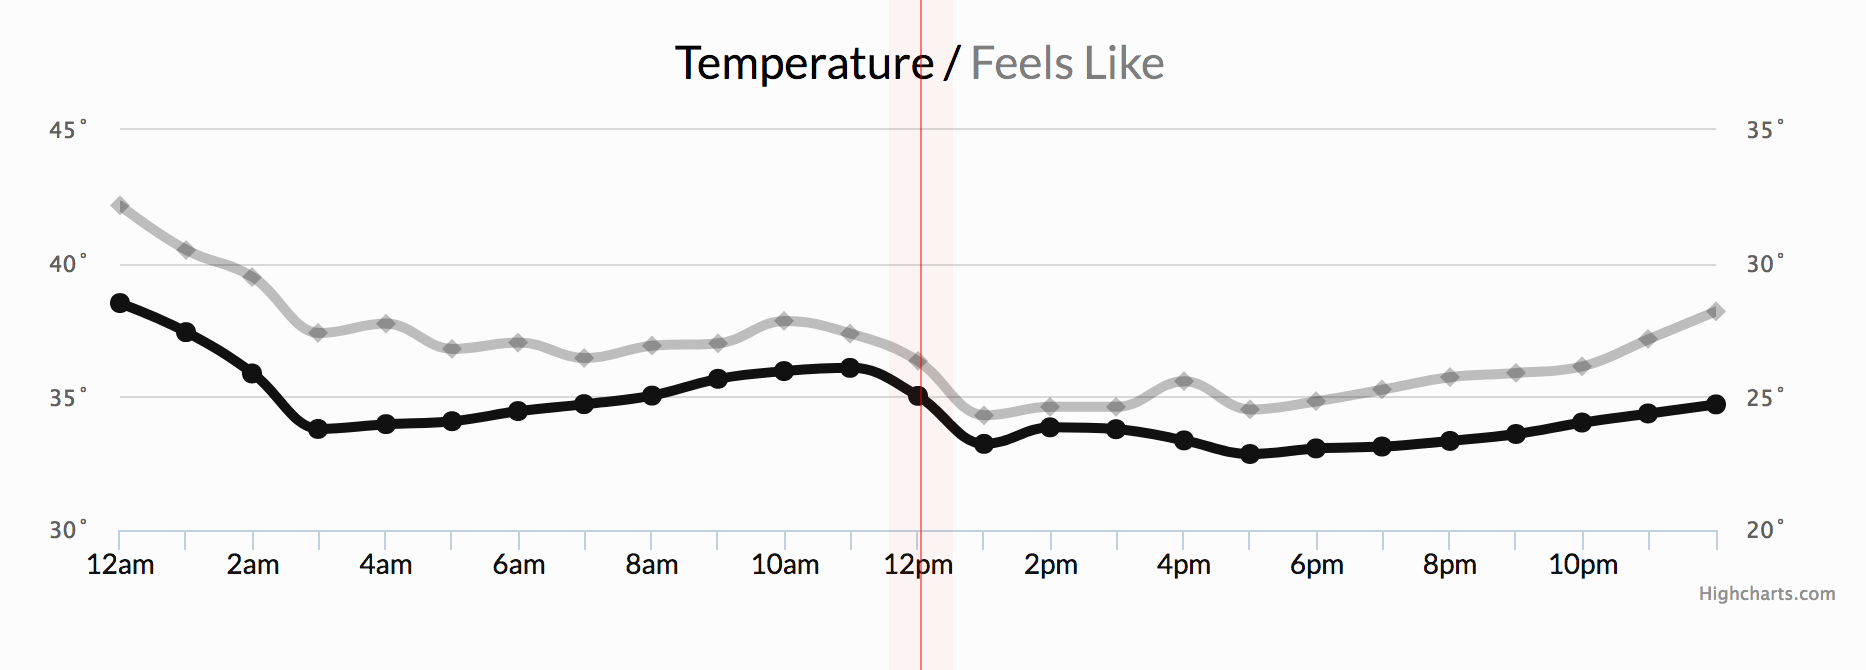
\includegraphics[width=\columnwidth]{figures/pt_br/dado_temporal}
  \caption{Exemplo de dados temporais: condições climáticas.
  O ponto em destaque representa um único registro de dados capturado em um instante específico.}
  \label{fig:temporal_data}
\end{figure}

\begin{figure}[ht]
  \centering
  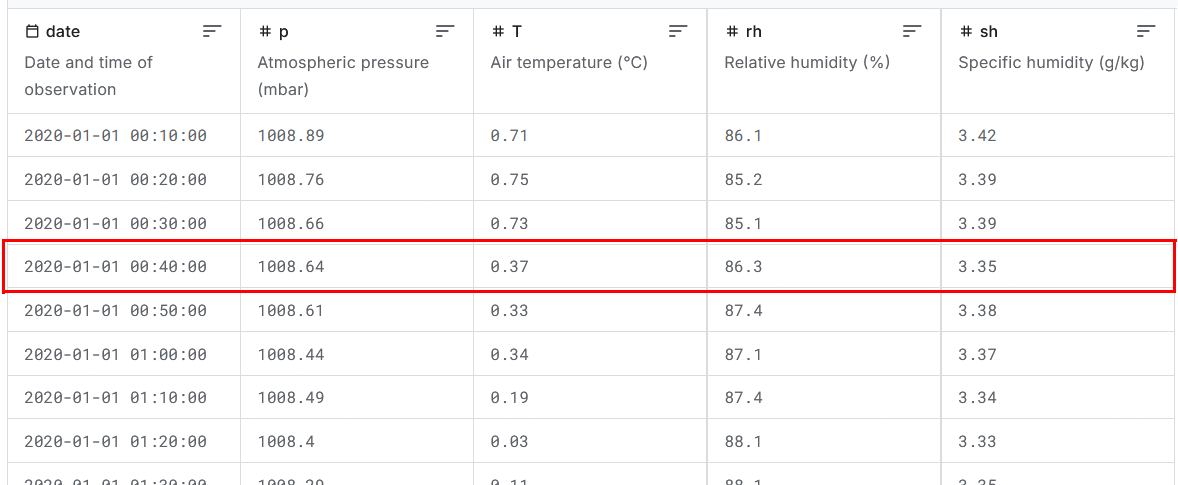
\includegraphics[width=\columnwidth]{figures/pt_br/registro_temporal}
  \caption{Exemplo de tabela em um BDST representando a série temporal climática.
  Cada linha corresponde a uma medição indexada por tempo.}
  \label{fig:tsdb_record}
\end{figure}

A Figura~\ref{fig:tsdb_record} mostra a tabela correspondente em um BDST, onde cada linha é um
registro indexado por tempo que captura pressão atmosférica, temperatura, umidade e outras
leituras em um momento específico.

Como explicado por~\cite{Ozsu2011}, uma série temporal normalmente consiste apenas em valores
numéricos, contínuos ou discretos. Isso torna possível modelar fluxos de dados que contêm apenas
valores numéricos como séries temporais, permitindo que técnicas de análise de séries temporais
sejam aplicadas a certos tipos de fluxos de dados. Uma característica fundamental é que os
conjuntos de dados de séries temporais são tipicamente utilizados em situações onde as medições,
uma vez realizadas, não são revisadas ou atualizadas, mas acumuladas: novos dados são
adicionados para cada parâmetro medido a cada novo instante de tempo, como observado
por~\cite{Dunning2014}.

A significância histórica da análise de séries temporais é notável, com exemplos que remontam
ao século XIX. \cite{Dunning2014} citam o trabalho pioneiro de Matthew Fontaine Maury, que
analisou diários de bordo de navios para criar cartas de vento e correntes, demonstrando como
a análise coletiva de dados de séries temporais acumulados ao longo de muitos anos em muitos
navios pode revelar padrões valiosos para a navegação marítima. Esse exemplo histórico ilustra
como os conjuntos de dados de séries temporais podem revelar tendências e padrões não aparentes
em medições pontuais.

No contexto moderno, os BDSTs enfrentam novos desafios devido ao volume, velocidade e variedade
dos dados gerados. O que costumava ser coletado em 10 minutos para alguns sistemas muito ativos
é agora gerado a cada segundo~\citep{Dunning2014}. Essa explosão no volume de dados exige novas
abordagens de armazenamento e acesso, tornando os bancos de dados NoSQL particularmente
adequados para essa escala. Para consultas baseadas em tempo em escalas muito grandes, esses
acessos podem ser implementados como varreduras grandes e contíguas, extremamente eficientes
quando os dados estão armazenados adequadamente em um banco de dados de séries temporais.

A arquitetura dos BDSTs modernos evoluiu consideravelmente. \cite{Dunning2014} descrevem três
abordagens principais para o armazenamento de séries temporais: (1) tabelas largas que
armazenam dados ponto a ponto; (2) um design híbrido misturando tabelas largas com armazenamento
em blob; e (3) inserção direta de blob a partir de um cache em memória, que pode atingir taxas
de ingestão até 1.000$\times$ mais rápidas que as abordagens ponto a ponto. Os BDSTs armazenam
múltiplas séries temporais de forma que consultas que recuperam dados de uma ou poucas séries
para um intervalo de tempo específico sejam particularmente eficientes~\citep{Dunning2014}.
Essa eficiência é alcançada por meio de estratégias de armazenamento que agrupam fisicamente
dados temporalmente próximos, habilitando operações eficientes de varredura sequencial.

As aplicações dos BDSTs são diversas e estão em expansão. No setor financeiro, a velocidade das
negociações e a necessidade de latência extremamente baixa tornam os BDSTs de alto desempenho
essenciais~\citep{Dunning2014}. No contexto IoT, os BDSTs ocupam uma posição central no fluxo de
dados de sensor à percepção que está mudando rapidamente como percebemos e entendemos o
mundo~\citep{Dunning2014}.

\subsubsection{Arquiteturas de Banco de Dados para Séries Temporais}

Os três bancos de dados comparados neste trabalho representam três arquiteturas distintas de
armazenamento para séries temporais, cada uma com diferentes compromissos entre vazão de escrita,
latência de leitura e consumo de recursos.

\textbf{Apache IoTDB}~\cite{wang2023iotdb} foi concebido especificamente para o domínio IoT.
Ele usa o TsFile~\citep{zhao2024tsfile}, um formato de arquivo colunar personalizado que armazena dados em blocos
ordenados com estatísticas de mínimo/máximo por bloco. As escritas são primeiro absorvidas em
um buffer em memória (memtable) gerenciado pela JVM e descarregadas para segmentos TsFile
de forma assíncrona. Essa estratégia de escrita diferida é similar a uma abordagem de
Log-Structured Merge Tree (LSM)~\citep{oneil1996lsm}, trocando garantias estritas de durabilidade por alta vazão
de escrita. A interface de ingestão nativa é um protocolo binário Thrift RPC
(SESSION\_BY\_TABLET), que submete tablets colunares tipados diretamente no buffer de escrita
com sobrecarga mínima. As estatísticas de mínimo/máximo armazenadas por bloco permitem a
eliminação antecipada de blocos que não correspondem ao predicado durante consultas de filtro
de valor, uma propriedade que se torna cada vez mais vantajosa à medida que o conjunto de
dados cresce~\citep{wang2023iotdb}.

\textbf{InfluxDB}~\cite{naqvi2017influxdb} usa um motor de armazenamento Time-Structured Merge
Tree (TSM), que organiza dados em blocos comprimidos ordenados por tempo. Assim como a árvore
LSM, o TSM armazena escritas em memória (cache TSM) e as compacta periodicamente em arquivos
imutáveis em disco. A ingestão de dados é realizada via API HTTP com protocolo de linha, onde
os clientes enviam texto no formato de protocolo de linha representando medições. As consultas
usam a linguagem Flux. O motor TSM mantém um Índice de Séries Temporais (TSI) para busca de
séries. A memória em processo do InfluxDB é dominada pelo cache TSM, pelo índice de séries e
pela sobrecarga do runtime Go~\citep{naqvi2017influxdb}.

\textbf{TimescaleDB} estende o PostgreSQL com otimizações para séries temporais~\citep{timescaledb}.
Sua estrutura de dados primária é a \textit{hipertabela}: uma tabela lógica que é
automaticamente particionada em \textit{blocos} físicos por intervalo de tempo. Consultas que
especificam um intervalo de tempo podem eliminar blocos automaticamente, tocando apenas as
partições relevantes. A função \texttt{time\_bucket()} fornece subamostragem nativa com
agregação por push-down. Como extensão do PostgreSQL, o TimescaleDB herda sua pilha de
armazenamento completa: todas as escritas passam pelo Write-Ahead Log (WAL) antes do
reconhecimento, o MVCC fornece isolamento por snapshot e os índices B-tree são mantidos em
colunas primárias e secundárias. Os índices BRIN (Block Range INdex) fornecem eliminação leve
baseada em intervalos para predicados de valor. O modelo de durabilidade baseado em WAL
oferece garantias fortes de segurança dos dados, mas introduz latência por escrita maior em
comparação com o buffering assíncrono do IoTDB e do InfluxDB.

\subsection{Benchmarks}

A avaliação de desempenho é um componente crítico do processo de seleção de banco de dados.
Como destacado por~\cite{Ramakrishnan2003}, quando um banco de dados cresce além da capacidade
do SGBD atual de fornecer desempenho satisfatório, a migração para um novo sistema deve ser
considerada. Os benchmarks são as principais ferramentas que permitem a comparação objetiva
entre os diferentes produtos disponíveis. Um único teste é insuficiente; como argumenta
\cite{Silberschatz2020}, um benchmark deve simular cargas de trabalho reais, pois cada produto
pode ter desempenho diferente dependendo da tarefa.

A complexidade dos SGBDs e as diferentes abordagens adotadas pelos fornecedores tornam os
benchmarks particularmente valiosos. Como observam~\cite{Ramakrishnan2003}, um SGBD é um
software complexo, e diferentes fornecedores podem ter como alvo diferentes segmentos de
mercado, otimizando certas partes de seus sistemas ou escolhendo projetos arquiteturais
distintos. Essa diversidade de abordagens e otimizações específicas torna a comparação direta
difícil sem instrumentos padronizados.

Quanto às características fundamentais de um bom benchmark,~\cite{Ramakrishnan2003} enumeram
três qualidades essenciais. Primeiro, \textit{portabilidade}: a capacidade de executar o
benchmark em diferentes plataformas e sistemas. Segundo, \textit{clareza}: garantir fácil
compreensão do que está sendo realmente medido. Terceiro, \textit{escalabilidade}: a adaptação
natural a instâncias maiores do problema. Além desses atributos básicos, bons benchmarks devem
medir tanto o desempenho máximo (expresso em métricas como transações por segundo) quanto a
relação custo-eficácia (dólares por transação por segundo) para cargas de trabalho típicas de
um domínio de aplicação específico. Foi precisamente para atender a essas necessidades que o
Transaction Processing Council (TPC) foi criado, com a missão de desenvolver benchmarks
padronizados para processamento de transações e sistemas de banco de dados.

\cite{Silberschatz2020} acrescenta uma observação importante sobre o cálculo correto de
desempenho: usar a média simples de vazões pode ser enganoso. O método correto é calcular o
tempo total para uma carga de trabalho mista e derivar a vazão média a partir disso, ou usar a
média harmônica, que reflete melhor a realidade quando há diferentes tipos de operações.

A literatura de benchmarks categoriza seus instrumentos em vários grupos~\citep{Ramakrishnan2003}.
Os benchmarks de \textit{Processamento de Transações Online} (TPC-A, TPC-B, TPC-C) definem
medidas padrão de transações por segundo e custo por transação. O TPC-C, o mais amplamente
utilizado, modela um ambiente complexo de armazém com cinco tipos de transação, exercitando uma
gama muito mais ampla de capacidades do sistema do que seus predecessores. Os benchmarks de
\textit{desempenho de consultas} (Wisconsin, AS3AP, TPC-D) avaliam o desempenho de consultas
relacionais, de simples a complexas para suporte a decisões. Os benchmarks de \textit{banco de
dados orientado a objetos} (001, 007, Bucky) medem sistemas orientados a objetos e
objeto-relacionais.

Para aplicação prática, os benchmarks devem ser interpretados com cuidado.
\cite{Ramakrishnan2003} alertam que métricas de desempenho de número único podem ser
demasiadamente simplistas para softwares complexos como um SGBD. Um bom benchmark deve incluir
um conjunto abrangente de tarefas cuidadosamente selecionadas para cobrir um domínio de
aplicação específico e para testar as capacidades do SGBD críticas para esse domínio. Os
analistas devem pesar as tarefas do benchmark de acordo com o quanto se assemelham às operações
críticas da aplicação pretendida; e, quando os benchmarks padrão não correspondem
suficientemente à carga de trabalho real, benchmarks personalizados que adaptem ou substituam
tarefas padrão por operações mais representativas devem ser considerados.

A reprodutibilidade é uma propriedade essencial, mas frequentemente negligenciada, dos benchmarks
de banco de dados. Como observado nos seis estudos de desempenho revisados neste trabalho, apenas um
fornece os scripts e configurações exatas necessárias para replicação
independente~\citep{pereira2023mulletbench}. Isso limita a capacidade
de validar resultados, comparar descobertas entre estudos e construir sobre trabalhos anteriores,
uma lacuna que este estudo aborda diretamente por meio de sua infraestrutura de benchmark
totalmente automatizada e publicamente disponível.
Além do compartilhamento de código, o isolamento de recursos entre os sistemas avaliados é
igualmente crítico: executar múltiplos motores de banco de dados simultaneamente no mesmo
hardware introduz artefatos de contenção de cache de páginas e E/S que podem inverter
conclusões reportadas~\citep{shapira2016pitfalls}.
